%!TEX program = xelatex
\documentclass{article}
\textwidth 156mm \textheight 220mm \oddsidemargin 5mm
\evensidemargin 5mm \topmargin -10mm
\usepackage{amsmath}
\usepackage{amsfonts,amssymb}
\usepackage{fontspec}
\usepackage{microtype}
\usepackage{setspace}
\usepackage{multirow}
\usepackage{blkarray}
\usepackage{tikz}
\usepackage{dsfont}
\usepackage{booktabs}
\usepackage{enumerate}
%\usepackage{indentfirst}
\usepackage{mathrsfs}
\usepackage{listings}
%\usepackage[usenames,dvipsnames]{xcolor}
\usepackage{epsf}
\usepackage[linesnumbered,boxed]{algorithm2e}
\usepackage[colorlinks,linkcolor=red]{hyperref}
\renewcommand\thesection{\Roman{section}}%\arabic{section}}
\renewcommand\thesubsection{\Roman{section.}\roman{subsection})}
\renewcommand\thesubsubsection{\arabic{subsubsection}.}
\defaultfontfeatures{Mapping=tex-text,Scale=MatchLowercase}
%\setmainfont{Citadel Script}
\setmainfont{Savoye LET}
%\setmainfont{Chalkboard}
%\setmainfont{Optima}
%\setmainfont{Apple Chancery}
\setmonofont{Optima}
\setsansfont{Optima}
%\renewcommand{\familydefault}{\sfdefault}
%\renewcommand{\footnotesize}{\sfdefault}
\setlength{\parskip}{\baselineskip}
\setlength{\parindent}{0em}
%%%%%%%%%%%Here is the configurations for Code%%%%%%%%%%%

\definecolor{mygreen}{rgb}{0,0.6,0}
\definecolor{mygray}{rgb}{0.5,0.5,0.5}
\definecolor{mymauve}{rgb}{0.58,0,0.82}
\lstset{
 backgroundcolor=\color{white}, 
 basicstyle = \footnotesize,       
 breakatwhitespace = false,        
 breaklines = true,                 
 captionpos = b,                    
 commentstyle = \color{mygreen}\bfseries,
 extendedchars = false,             
 frame =shadowbox, 
 framerule=0.5pt,
 keepspaces=true,
 keywordstyle=\color{blue}\bfseries, % keyword style
 language = C++,                     % the language of code
 otherkeywords={string}, 
 numbers=left, 
 numbersep=5pt,
 numberstyle=\tiny\color{mygray},
 rulecolor=\color{black},         
 showspaces=false,  
 showstringspaces=false, 
 showtabs=false,    
 stepnumber=0,         
 stringstyle=\color{mymauve},        % string literal style
 tabsize=2,          
 title=\lstname                      
}

%%%%%%%%%%%%%%%%%%%%%%%%%%%%%%%%%%%%%%%%%%%%

\begin{document}
\renewcommand\arraystretch{1.5}


\thispagestyle{empty}

\begin{center}
\begin{large}
\begin{figure}[!htbp]
\centering

\includegraphics[width=0.7\textwidth]{Logo2.png}
\end{figure}
\hrule
\vspace*{0.25cm}
\sc{UM--SJTU Joint Institute \vspace*{0.3em}} \\ 
VE281 Data Structure and Algorithm\\
\end{large}
\hrulefill

\vspace*{5cm}

\begin{Large}
\sc{{Project 3 Report}} \\
\end{Large}
\vspace*{2em}
\begin{large}
\sc{{Tianze Wang, 515370910202}}
\end{large}
\end{center}
\newpage
\setmainfont{Optima}
\setcounter{page}{1}
\section{Introduction}
\par In this project, we implement the data structure of priority queue in the means of 
\begin{itemize}
\item Binary Heap
\item Unsorted Heap
\item Fibonacci Heap
\end{itemize}
And we will discuss and compare the performance of them.
\section{A table comparing 2 sort methods}
\par To compare the performance, we use seven maps with distinct and significant differences in size to compare. The result is shown as below.(The testcase means the single side of a map, namely 5 corresponds to 25 in map size)
% Table generated by Excel2LaTeX from sheet '工作表1'
% Table generated by Excel2LaTeX from sheet '工作表1'
\begin{table}[htbp]
  \centering

    \begin{tabular}{lrrrrrrrrr}
    Testcase & 5     & 10    & 15    & 20    & 25    & 30    & 50    & 100   & 1000 \\
    Binary Heap & 2.40E-05 & 2.60E-05 & 8.30E-05 & 0.000101 & 0.000165 & 0.000197 & 0.000663 & 0.001711 & 0.258891 \\
    Fib Heap & 2.40E-05 & 8.00E-05 & 1.25E-04 & 0.000201 & 0.000402 & 4.85E-04 & 8.64E-04 & 2.82E-03 & 5.70E-01 \\
    Unsorted Heap & 2.20E-05 & 6.00E-05 & 6.40E-05 & 9.70E-05 & 0.000202 & 0.000241 & 0.001119 & 0.004743 & 5.21586 \\
    \end{tabular}%
\end{table}%

To make intuitive, we use log for both axis.
% Table generated by Excel2LaTeX from sheet '工作表1'
\begin{table}[htbp]
  \centering

    \begin{tabular}{lrrrrrrrrr}
    Testcase & 0.70  & 1.00  & 1.18  & 1.30  & 1.40  & 1.48  & 1.70  & 2.00  & 3.00  \\
    Binary Heap & -4.62  & -4.59  & -4.08  & -4.00  & -3.78  & -3.71  & -3.18  & -2.77  & -0.59  \\
    Fib Heap & -4.62  & -4.10  & -3.90  & -3.70  & -3.40  & -3.31  & -3.06  & -2.55  & -0.24  \\
    Unsorted Heap & -4.66  & -4.22  & -4.19  & -4.01  & -3.69  & -3.62  & -2.95  & -2.32  & 0.72  \\

    \end{tabular}%
\end{table}%
\newpage
And the result is shown here.

\begin{figure}[!htbp]
\centering
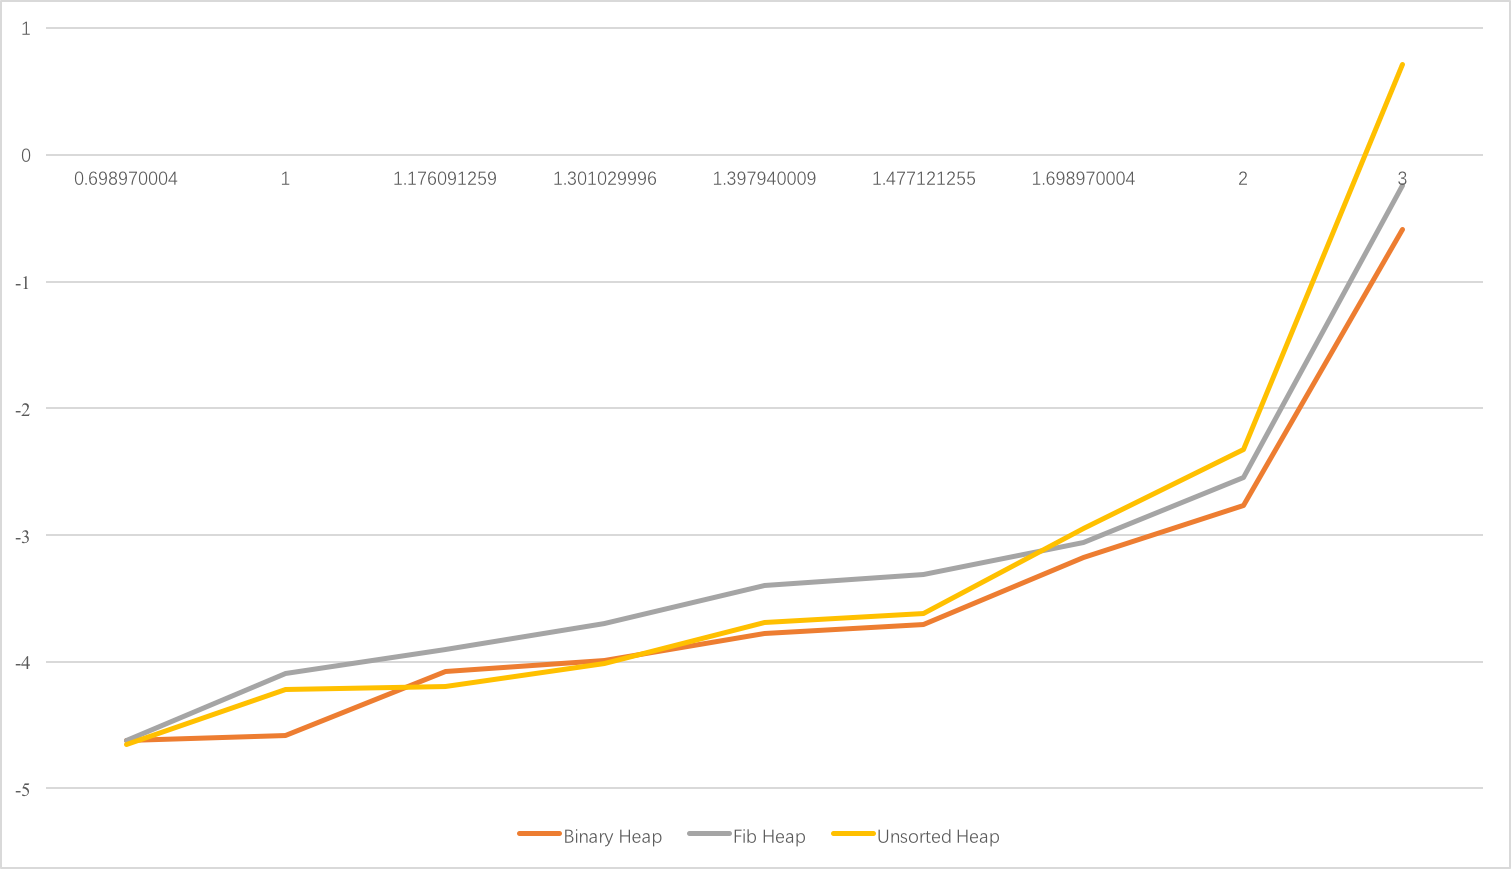
\includegraphics[width= \textwidth]{Pic1.png}
\end{figure}

\section{Discussion and Conclusion}
From the figure and the result, we can derive that:
\begin{itemize}
\item Binary heap performs best in any case.
\item Unsorted heap is quick when the data amount is not so big, but slow when it becomes big enough.
\item Fibonacci heap is slow at small data amount, but fast as binary heap when it becomes big.
\end{itemize}


\end{document}